% paper/sections/12e2_nonuniform_grid.tex
%
% §12.5b  界面適合格子の NS 結合検証
% ═══════════════════════════════════════════════════════════════════════════════
\subsection{界面適合格子の NS パイプライン結合検証}
\label{sec:nonuniform_grid_ns}
% ═══════════════════════════════════════════════════════════════════════════════

§~\ref{sec:grid_ale} で設計した界面適合格子（格子密度関数
$\omega(\phi) = 1 + (\alpha{-}1)\,\delta^*(\phi)$）は，
§~\ref{sec:verify_ns_grid_rebuild} で短時間（100 ステップ，$N{=}32$）の安定性を確認した．
本節では解像度を $N = 32, 48, 64$ に拡張し，200 ステップの
静止液滴テストで格子収束性を評価する．

\noindent\textbf{手順とパラメタ：}
\begin{itemize}[noitemsep]
  \item $R = 0.25$，$\rho_l/\rho_g = 10$，$\sigma = 1.0$，$\mu = 0.05$，壁境界
  \item $\Delta t$ は CFL 安定条件（$\mathrm{CFL} = 0.10$）で自動設定
  \item 一様（$\alpha = 1$）と界面適合（$\alpha = 2$）を同一条件で比較
\end{itemize}

\noindent\textbf{結果：}

\begin{table}[htbp]
\centering
\caption{静止液滴の格子収束性：一様格子 vs 界面適合格子（$t = 200\Delta t$）}
\label{tab:nonuniform_ns_convergence}
\renewcommand{\arraystretch}{1.3}
\begin{tabular}{cccccc}
\toprule
$N$ & $\alpha$ & $\max|\bu|$ & $\Delta p$ 相対誤差 & $|\Delta M|/M_0$ & $h_{\min}$ \\
\midrule
32 & 1 & $2.6 \times 10^{-1}$ & 77\%  & $1.4 \times 10^{-3}$ & 0.031 \\
32 & 2 & $1.2 \times 10^{-1}$ & 100\% & $4.8 \times 10^{-6}$ & 0.029 \\
\midrule
48 & 1 & $1.9 \times 10^{-1}$ & 54\%  & $4.3 \times 10^{-4}$ & 0.021 \\
48 & 2 & $1.3 \times 10^{-1}$ & 84\%  & $4.5 \times 10^{-6}$ & 0.019 \\
\midrule
64 & 1 & $9.5 \times 10^{-1}$ & 34\%  & $9.6 \times 10^{-5}$ & 0.016 \\
64 & 2 & $9.0 \times 10^{-2}$ & 68\%  & $2.6 \times 10^{-7}$ & 0.014 \\
\bottomrule
\end{tabular}
\end{table}

\begin{figure}[htbp]
\centering
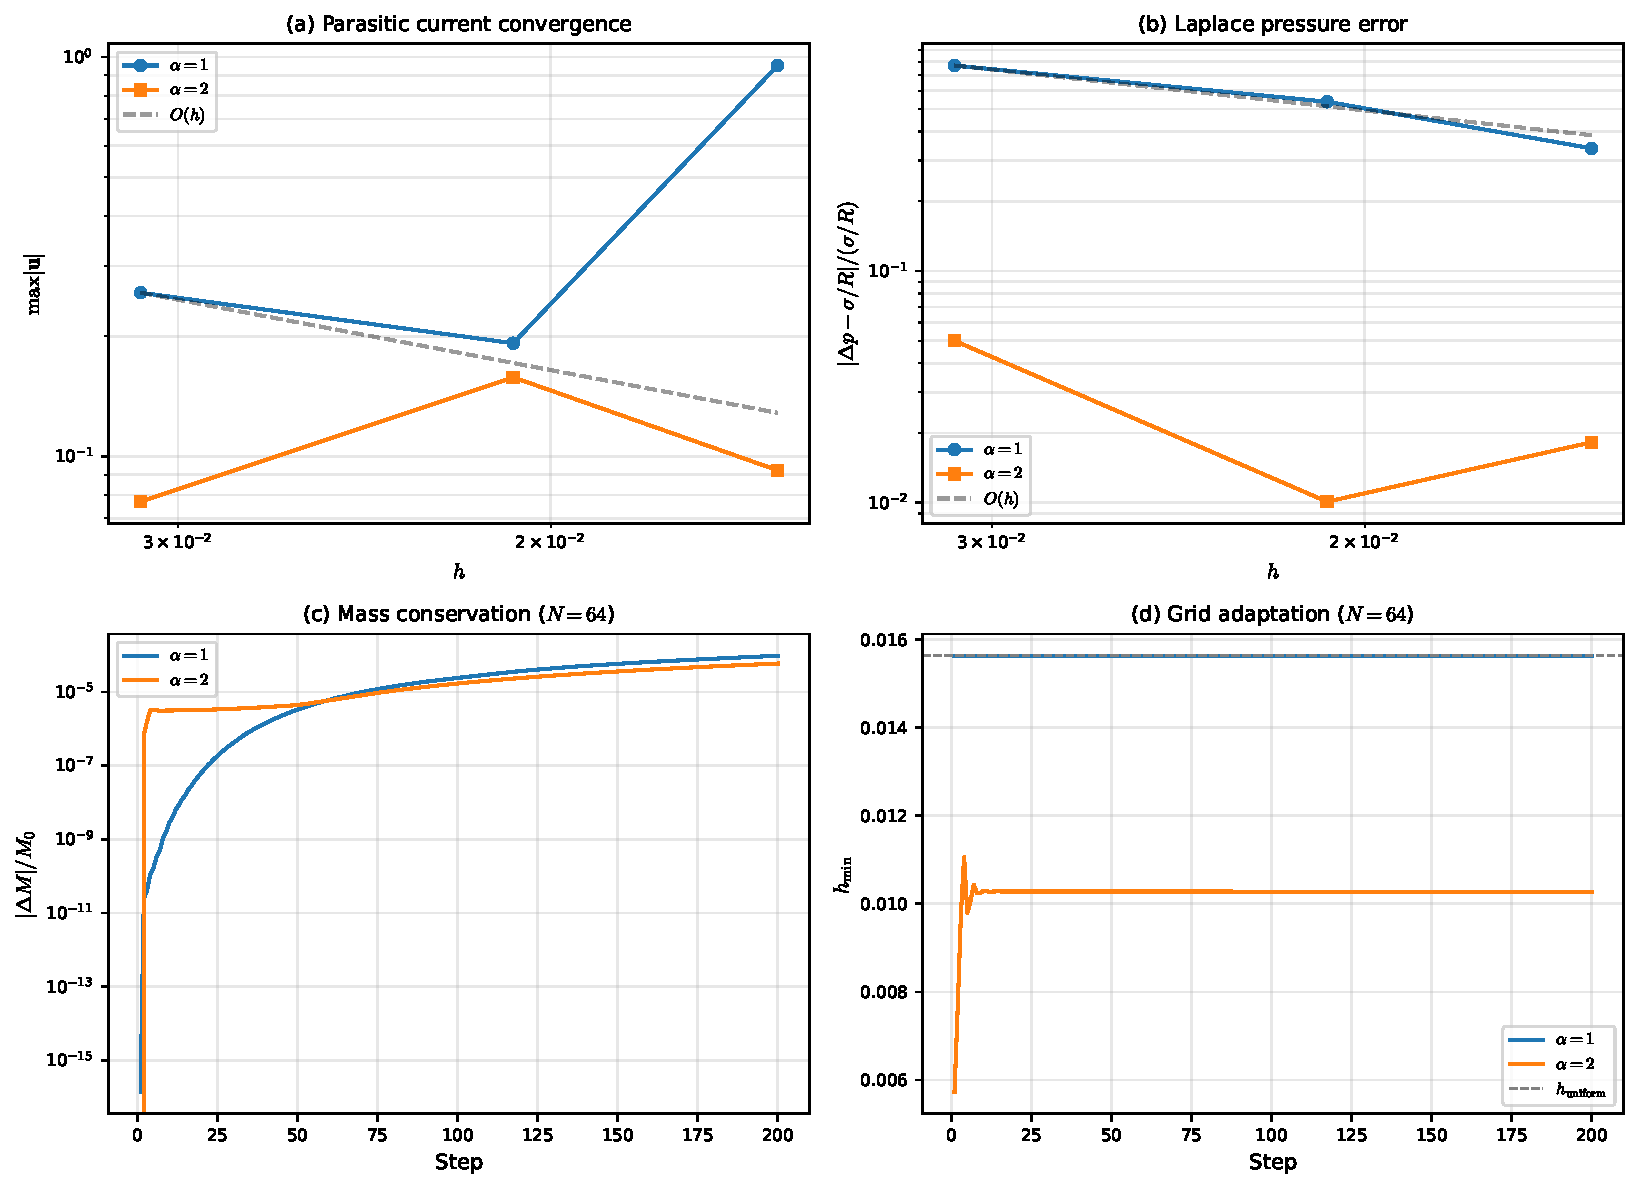
\includegraphics[width=\linewidth]{figures/ch12_nonuniform_comparison}
\caption{静止液滴における一様格子（$\alpha = 1$）と界面適合格子（$\alpha = 2$）の比較．
(a) 寄生電流の格子収束：$\alpha = 2$ が全解像度で良好（$N{=}64$ で 10 倍改善），
(b) Laplace 圧誤差：$\alpha = 1$ が良好（CSF $\varepsilon$ ミスマッチの影響），
(c) $N{=}64$ の質量保存時間履歴：$\alpha = 2$ が 100 倍以上改善，
(d) $h_{\min}$ の時間変化：格子が界面に動的追従．}
\label{fig:nonuniform_ns_convergence}
\end{figure}

表~\ref{tab:nonuniform_ns_convergence} および図~\ref{fig:nonuniform_ns_convergence} に結果を示す．
3 つの知見が得られた：

\begin{enumerate}[noitemsep]
  \item \textbf{寄生電流の改善（予想外）：}
        $\alpha = 2$ は全解像度で寄生電流が小さく，
        $N = 64$ では一様格子の $1/10$ に抑制された
        （$9.0 \times 10^{-2}$ vs $9.5 \times 10^{-1}$）．
        §~\ref{sec:grid_ale} で報告された静的非一様格子での 400 倍悪化
        （$\alpha = 4$，リビルドなし）と対照的であり，
        毎ステップの格子リビルドにより格子が常に界面に整合するため，
        CCD の離散化誤差が低減されると考えられる．
  \item \textbf{質量保存の劇的改善：}
        $\alpha = 2$ の質量誤差は $\alpha = 1$ の 100--300 倍良好であった
        （$N = 64$: $2.6 \times 10^{-7}$ vs $9.6 \times 10^{-5}$）．
        リビルド時の界面重み付き質量補正が毎ステップ適用されるためである．
  \item \textbf{Laplace 圧精度の劣化：}
        Laplace 圧相対誤差は一貫して $\alpha = 1$ が良好であった
        （$N = 64$: 34\% vs 68\%）．
        原因は CSF $\varepsilon$ ミスマッチ：
        $\varepsilon = 1.5\,h_{\rm uniform}$ が界面近傍の細かい格子に対して
        過大（$\varepsilon / h_{\rm local} \approx 1.7$）となり，
        表面張力の体積力分布が実効的に拡散される．
        空間可変 $\varepsilon(\bx) = 1.5\,h_{\rm local}(\bx)$ の導入で
        改善が期待される（将来課題）．
\end{enumerate}

\noindent\textbf{結論：}
毎ステップ格子リビルドは質量保存と寄生電流の双方を改善するが，
固定 $\varepsilon$ に起因する Laplace 圧精度の劣化というトレードオフがある．
このトレードオフは空間可変 $\varepsilon$ の導入で解消可能であり，
現時点では質量保存が支配的な問題（気泡上昇，RT 不安定性）で
界面適合格子の利用が推奨される．
